\documentclass[conference]{IEEEtran}
\usepackage{cite}
\usepackage{amsmath,amssymb,amsfonts}
\usepackage{algorithmic}
\usepackage{graphicx}
\usepackage{textcomp}
\usepackage{xcolor}
\def\BibTeX{{\rm B\kern-.05em{\sc i\kern-.025em b}\kern-.08em
    T\kern-.1667em\lower.7ex\hbox{E}\kern-.125emX}}
\begin{document}

\title{Nanuda: A Group Expenses Manager}

\author{\IEEEauthorblockN{1\textsuperscript{st} Abia Herlianto}
\IEEEauthorblockA{\textit{School of Computer Science} \\
\textit{BINUS University}\\
\textit{Team MONEY}\\
Jakarta, Indonesia \\
abiaph@live.com}
\and
\IEEEauthorblockN{2\textsuperscript{nd} Hugo Ravé}
\IEEEauthorblockA{\textit{General Engineering} \\
\textit{ESILV PARIS-LA DEFENSE}\\
\textit{Team MONEY}\\
Paris, France \\
hugorave07@gmail.com}
\and
\IEEEauthorblockN{3\textsuperscript{rd} Nadya Hartanto}
\IEEEauthorblockA{\textit{School of Information Systems} \\
\textit{BINUS University}\\
\textit{Team MONEY}\\
Jakarta, Indonesia \\
ndhartanto1@gmail.com}
}

\maketitle

\begin{abstract}
Users create a "group" composed of either one person (themselves) or several people. Users then invite these people to the group. Users add expenses and split the costs with either all, some, or no members of the group. Users can categorise and add descriptions for each expense. Users can also customise how the costs are split. Users can see a summary of how much they owe to others, how much others owe to others, as well as statistics of their expenses based on categories. The summary of how much users owe changes as users spend and pay.
\end{abstract}

\begin{IEEEkeywords}
expenses, finance, management
\end{IEEEkeywords}

\begin{center}
\begin{tabular}{|p{6em}|p{5em}|p{10em}|}
\hline
\textbf{Role} & \textbf{Name} & \textbf{Task Description etc.} \\
\hline
\textbf{User/Customer} & Nadya Hartanto & Tests the application for bugs and issues. Provides feedback to the Development Manager.
Also provides feedback on UX and UI quality. \\
\hline
\textbf{Software Developer} & Abia Putrama Herlianto & Implements software based on design. Fixes bugs and issues. \\
\hline
\textbf{Development Manager} & Hugo Ravé & Designs software based on requirements and feedback from User/Customer. Organises, schedules, and manages development. \\
\hline
\end{tabular}
\end{center}

\section{Introduction}
When there are shared expenses in a group, it can be complicated to split the costs and gather the money that each person should pay. The usual solution is to have one or several individuals cover the cost of the entire group, and from there the remaining group members would pay their share to those who covered the cost.

The problem that arises from this is keeping track of these expenses. This is especially true for groups that meet regularly; for example, a group of friends going on a trip. Keeping track of who covered what for how much and who owes whom how much can quickly get out of hand. The solution that we propose is a simple application where these expenses can be organised, viewed, and accessed by all members of a certain group.

The name Nanuda comes from Korean 나누다, meaning 'to divide (up), to split (up)'. The name was chosen because our own experiences in splitting expenses in Korea was the reason we thought up of the idea.

There are several existing applications that perform a similar function, with different individual features. These include Tricount and Sesterce.
\\
\\
1. Tricount
\begin{figure}[htbp]
    \centerline{
\includegraphics[width=50mm,scale=0.5]{img/logo-tricount.png}}
    \caption{Tricount}
    \label{fig:my_label}
\end{figure}
\\
(Data from Google Play Store) \\
Rating: 4.8 stars \\
Downloads: 1 million+ \\
Key features: Users can share a simple link to share their expenses. Members of a group can add expenses and see the balance. Expenses can be shared unevenly. Tricount works both offline and online, with logging in being optional. It also has both a mobile app and a website.
\\
\\
2. Sesterce
\begin{figure}[htbp]
    \centerline{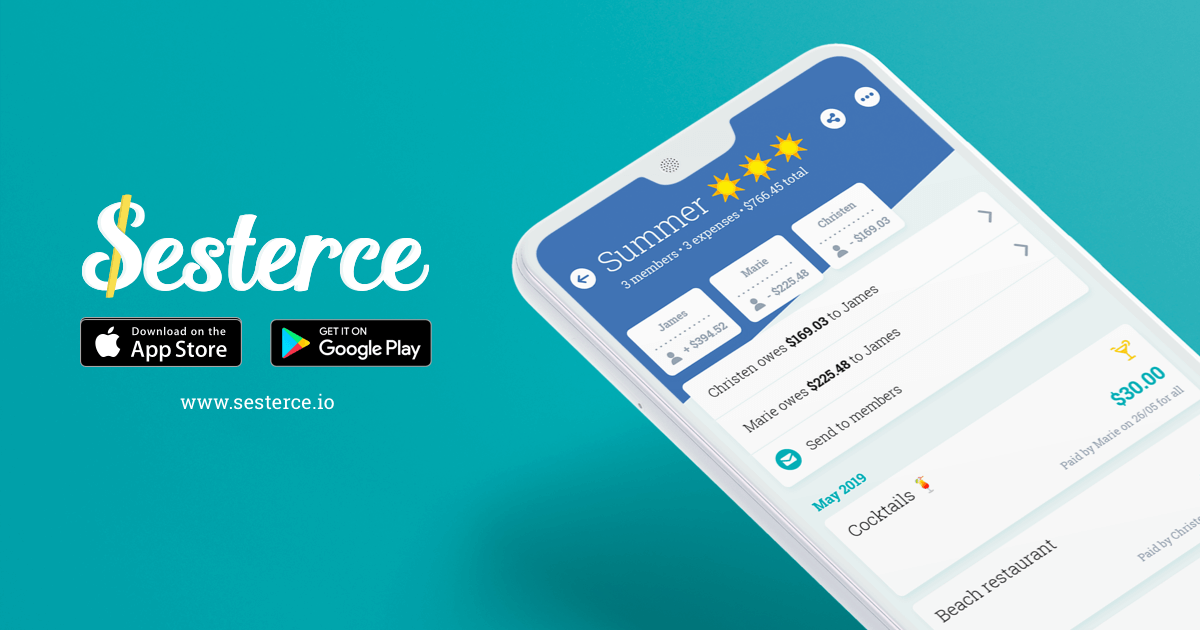
\includegraphics[width=50mm,scale=0.5]{img/logo-sesterce.png}}
    \caption{Sesterce}
    \label{fig:my_label}
\end{figure}
\\
(Data from Google Play Store) \\
Rating: 4.7 stars \\
Downloads: 5,000+ \\
Key features: Similar to Tricount, users can join a single group and add expenses, keeping track of all bills and costs. Sesterce is completely anonymous with no login or email required. In addition, Sesterce allows the addition of custom categories for expenses, the option to view statistics, and exporting all the data to a .csv file.

\section{Requirements}
\begin{enumerate}
    \item \textbf{Expenses Tracking}: Users can add expenses, who paid for them, who owes whom, and how much.
    \item \textbf{Detailed Information}: Users can categorise expenses as well as add names and descriptions.
    \item \textbf{Cost-Splitting Calculator}: An automatic calculator that calculates how much each person needs to pay the person who covers the cost. It should include default calculations such as evenly split. It should also include the option to manually specify who should pay how much.
    \item \textbf{Multiple Currency Support}: Users can specify what currency to be used in the group as well as per expense.
    \item \textbf{Summaries}: Users can see how much they owe or are owed in summary. This also includes information on how much they owe to others per person in total (e.g. I owe in total 100 dollars, 20 to A, and 80 to B). Users can also see the same information for other members of the group.
    \item \textbf{Statistics}: Users can see the statistics of how much is spent based on category. Users can also see the rate of spending.
    \item \textbf{Lightweight, Simple UI}: The app should be lightweight and easy to use, as well as easy on the eyes. It should show what the user needs to see, no more, no less.
\end{enumerate}

\end{document}
